\chapter{Data}\label{ch:data}
The data is provided by Östgötatrafiken, and follows a certain format.
A single observation comprises a timestamp, GPS position, and a
specific event type. Depending on the event type,
additional fields will be present. There are 22 different event types,
but only four of them are relevant for the thesis project.
The observation format is illustrated in 
Figure~\ref{fig:example-observation}, and event specific fields are
illustrated in Figure~\ref{fig:example-observation}.
\begin{figure}
  \centering
  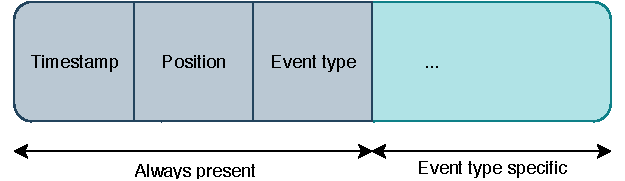
\includegraphics[scale=0.8]{observation-format}
  \caption{Format of an observation. Includes only the
    fields relevant to this thesis project.}\label{fig:example-observation}
\end{figure}

\begin{figure}
  \centering
  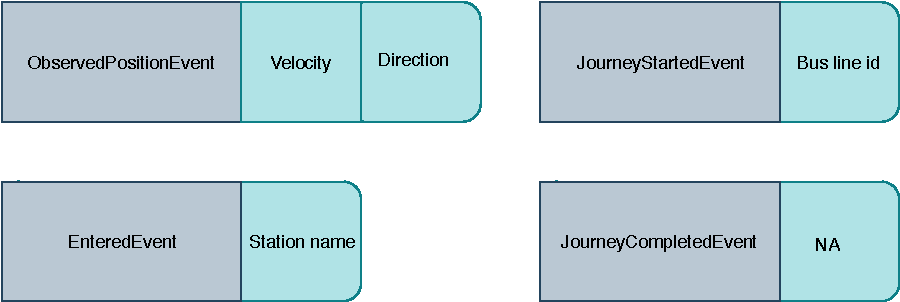
\includegraphics[scale=0.8]{event-types-format}
  \caption{Format of fields specific to event types used in this
    thesis project.}\label{fig:event-types-format}
\end{figure}
All data is sent from either buses or trains. However since the thesis
project is limited to trains, observations sent from trains are
discarded. A summary of the different even types, including when they
are sent can be seen in Table~\ref{tbl:event-sent}.

\begin{table}
  \centering
  \caption{Summary of the event types used in the thesis project.}\label{tbl:event-sent}
\resizebox{14.5cm}{!}{
  \begin{tabular}{ |l|l|l| }
    \hline
    Event type & Additional data & Sent \\ 
    \hline
    ObservedPositionEvent &  Velocity, Direction & Approximately every second. \\
    EnteredEvent & Station name & When driving sufficiently close to a bus stop. \\ 
    JourneyStartedEvent & Bus line id & When a bus is assigned a journey, before it
                                        leaves the station. \\
    JourneyCompletedEvent & & When a bus enters the final bus stop on a
                              bus line. \\ 
    \hline
  \end{tabular}
}
\end{table}

Since the ObservedPositionEvent is sent every second it causes
observations to spatially cluster when a bus is standing still. This
happens frequently at bus stops, when a bus stops to pick up or drop
off passengers, but also at the start of the journey. This is because
a bus is assigned a journey several minutes before actually
leaving. A heat map of observations can be seen in
Figure~\ref{fig:bus203-heatmap} which shows this phenomenon.

\begin{figure}
  \centering
  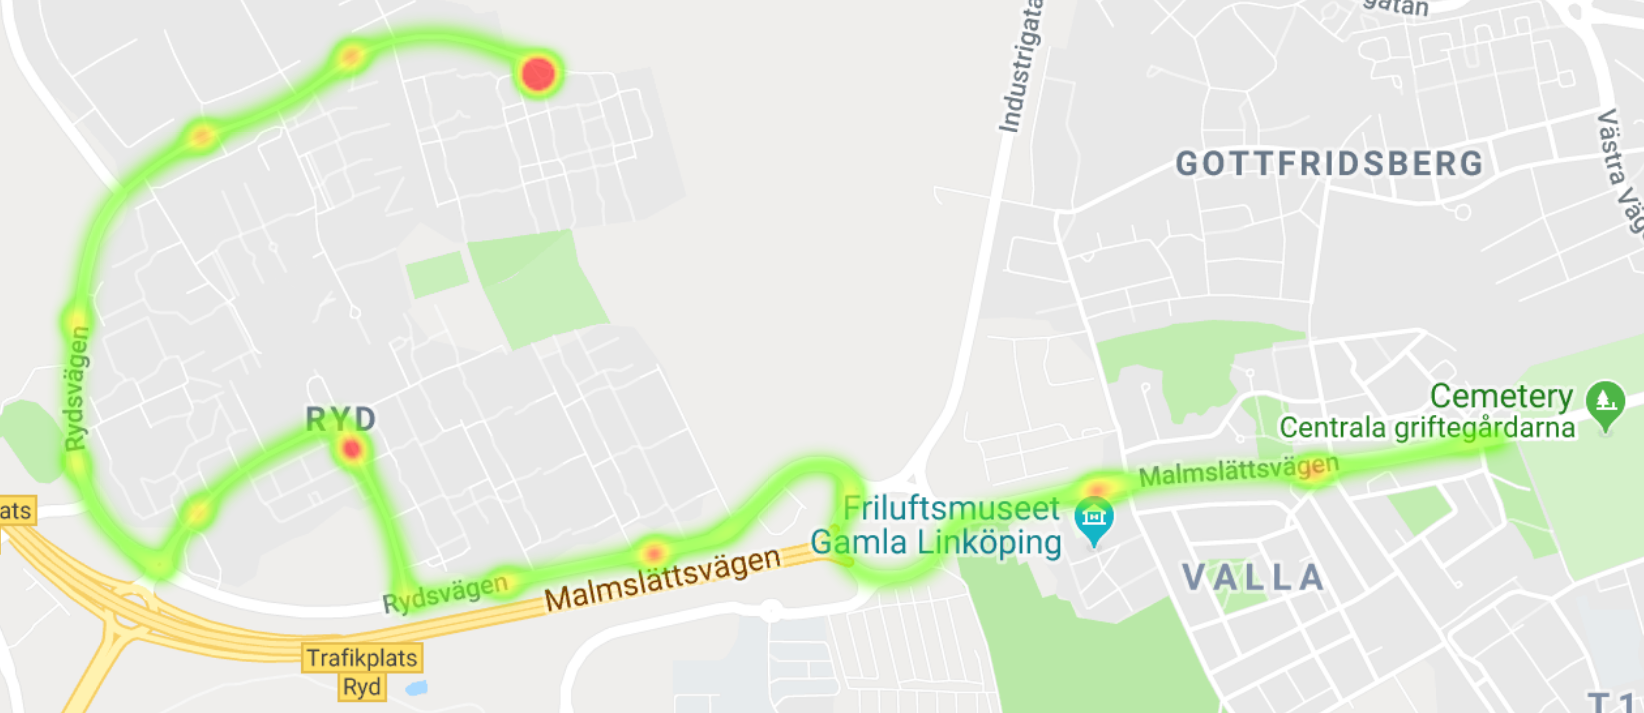
\includegraphics[scale=0.25]{bus203-heatmap}
  \caption{Heat map of observations collected in the beginning of bus line 3. 
    Red indicates areas with high frequency of observations and green indicates areas with
    low frequency. The start of the route is in the top left, where
    the frequency of observations is very high. }\label{fig:bus203-heatmap}
\end{figure}

%\[[2018-02-16T00:00:10.0000000+01:00, 2, ObservedPositionEvent, 2568098808, Normal, 0.0, Train, otraf.se, 9031005990006067, 6067, 58.5866813659668,16.2035980224609, 58.5866813659668,16.2035980224609, 291.700012207031, 0, 2500714]\]

% The provided data consists of one file per day, with a total of 92 days between February and April in 2018. Each file has an approximate size of 5 GB, with around 2.4 million observations per file. Within these files are logs over the \textit{events}, which each bus sends throughout the day. The events represent different states of the bus, and there are over 20 different event-types. For this project, only four event-types were needed to successfully extract complete journeys that could be used as input for our models. These four events and their usage are listed below:\\
% \begin{description}
% \item[ObservedPositionEvent:] Is sent by buses with a frequency of 1Hz. This event contains the GPS data, speed, and direction (angle) of a given bus.
% \item[EnteredEvent:] Is triggered when the bus is within a certain distance to a bus station. This event is used to split a journey into segments.
% \item[JourneyStartedEvent:] Is triggered when the bus is assigned a new journey. This event is used to determine which line a bus is currently serving.
% \item[JourneyCompletedEvent:] Is triggered when the bus has completed a journey. This event is used as a flag to determine when a journey has ended.
% \end{description}


%Explain data format
%Explain one observation per second
%Explain the clusters at stops
